\documentclass{article}
\usepackage[T1]{fontenc}
\usepackage{lmodern}
\usepackage{graphicx}
\usepackage{amsmath,amssymb}
\usepackage[a4paper,margin=2cm]{geometry}
\usepackage[absolute,overlay]{textpos}
\setlength{\TPHorizModule}{1mm}
\setlength{\TPVertModule}{1mm}
\usepackage[indonesian]{babel}
\usepackage{hyperref}
\setlength{\emergencystretch}{2em}
% unit: Halaman 19

\begin{document}

% === Halaman 19 (llm) ===

\vspace{273.24mm}

\vspace{10mm}
\textbf{Gambar 5. Diagram komputasi fungsi $f$:}

% deskripsi: Diagram alir komputasi fungsi f dalam algoritma DES, menunjukkan proses ekspansi, XOR dengan kunci, substitusi S-box, dan permutasi.
% bbox normalisasi: [0.0000, 0.0000, 0.9800, 0.9200]
\begin{textblock*}{205.80mm}(0.00mm,0.00mm)
\noindent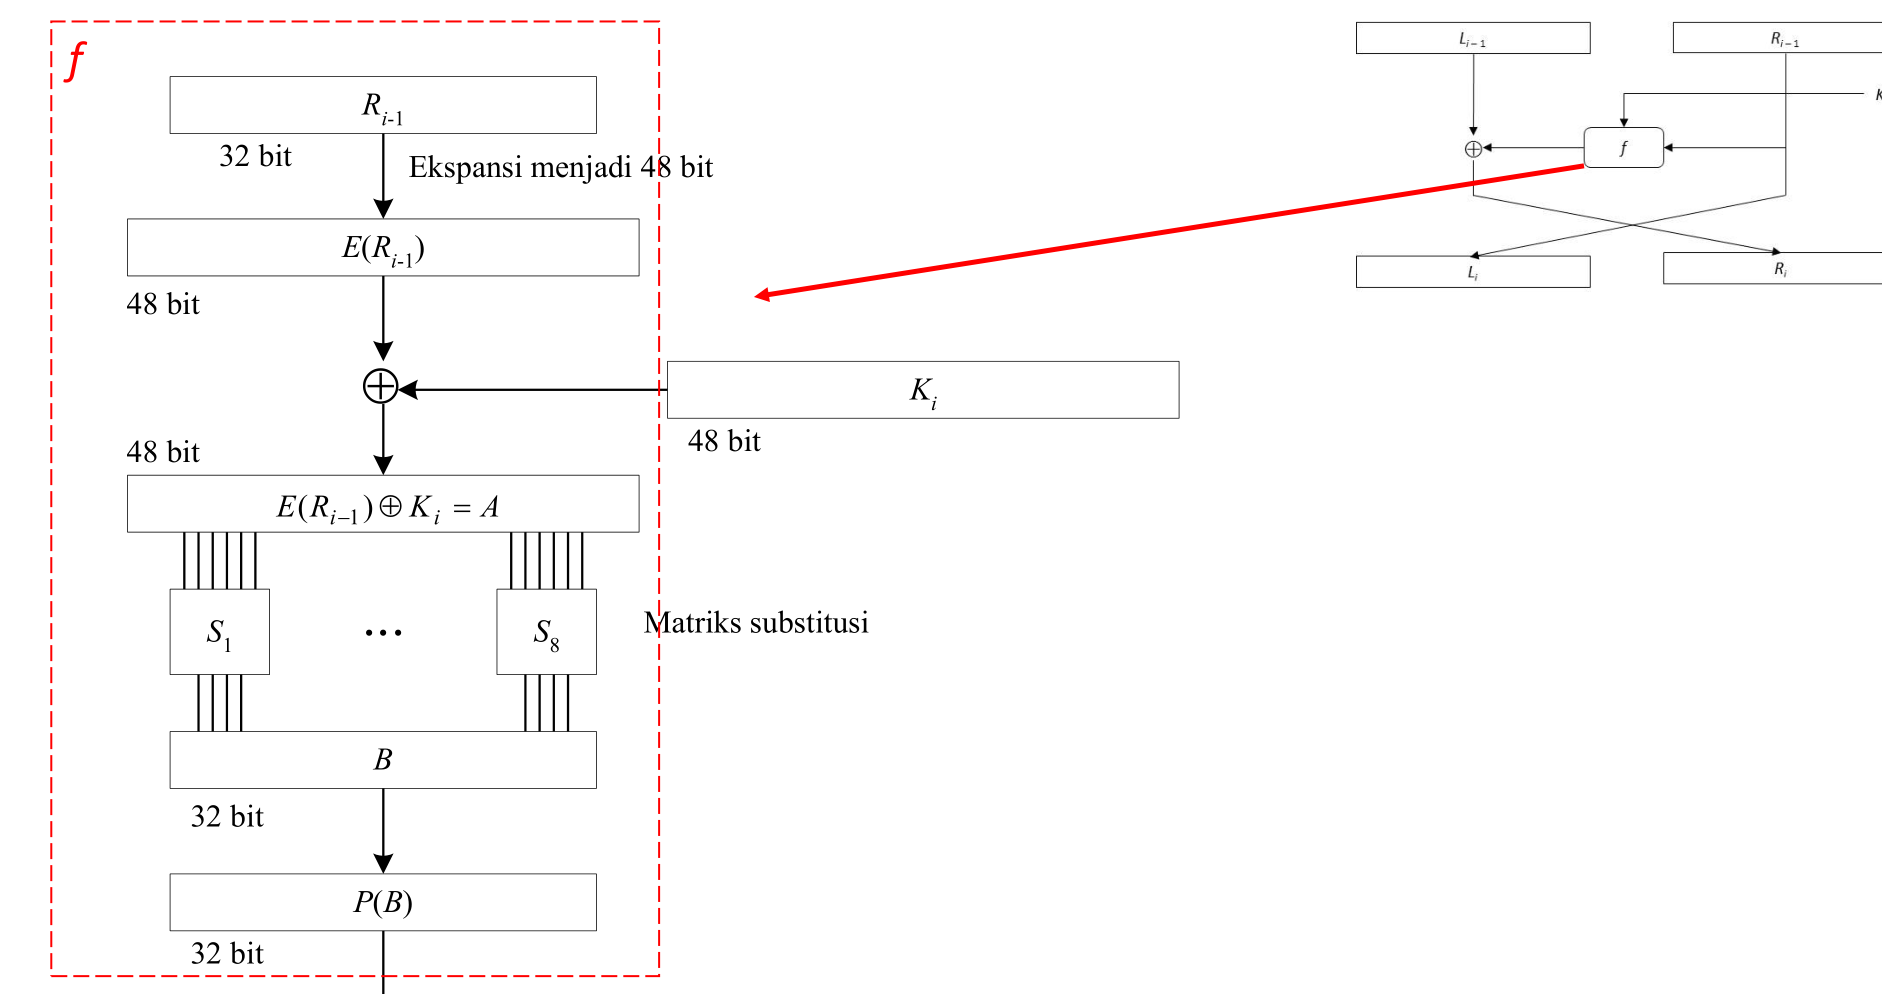
\includegraphics[width=205.80mm,height=273.24mm]{../../images/llm/page_019_img_01.png}%
\end{textblock*}

\end{document}
